% Created by tikzDevice version 0.12.3.1 on 2023-03-16 10:51:15
% !TEX encoding = UTF-8 Unicode
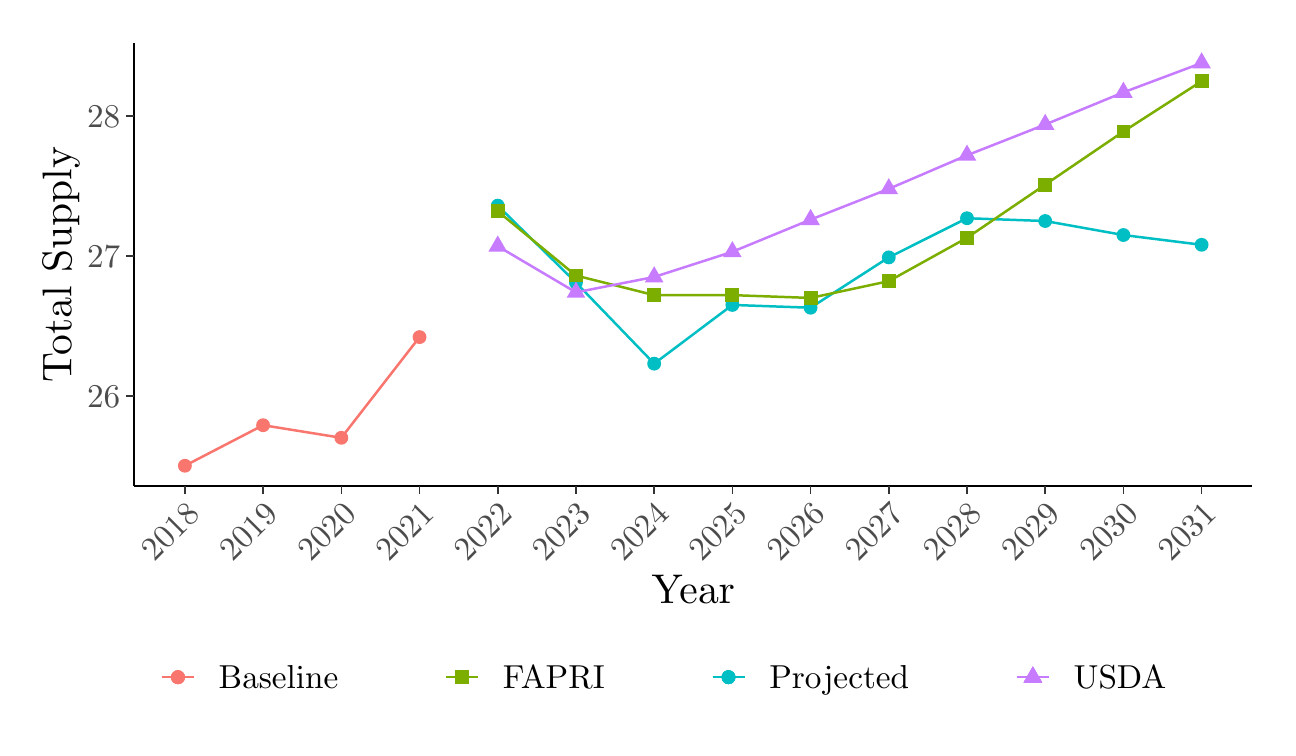
\begin{tikzpicture}[x=1pt,y=1pt]
\definecolor{fillColor}{RGB}{255,255,255}
\path[use as bounding box,fill=fillColor,fill opacity=0.00] (0,0) rectangle (448.07,252.94);
\begin{scope}
\path[clip] (  0.00,  0.00) rectangle (448.07,252.94);
\definecolor{drawColor}{RGB}{255,255,255}
\definecolor{fillColor}{RGB}{255,255,255}

\path[draw=drawColor,line width= 0.6pt,line join=round,line cap=round,fill=fillColor] (  0.00,  0.00) rectangle (448.07,252.94);
\end{scope}
\begin{scope}
\path[clip] ( 38.44, 87.36) rectangle (442.57,247.45);
\definecolor{fillColor}{RGB}{255,255,255}

\path[fill=fillColor] ( 38.44, 87.36) rectangle (442.57,247.44);
\definecolor{drawColor}{RGB}{248,118,109}

\path[draw=drawColor,line width= 0.9pt,line join=round] ( 56.81, 94.64) --
	( 85.07,109.29) --
	(113.34,104.74) --
	(141.60,141.13);
\definecolor{fillColor}{RGB}{248,118,109}

\path[fill=fillColor] ( 56.81, 94.64) circle (  2.50);

\path[fill=fillColor] ( 85.07,109.29) circle (  2.50);

\path[fill=fillColor] (113.34,104.74) circle (  2.50);

\path[fill=fillColor] (141.60,141.13) circle (  2.50);
\definecolor{drawColor}{RGB}{0,191,196}

\path[draw=drawColor,line width= 0.9pt,line join=round] (169.86,188.63) --
	(198.12,160.83) --
	(226.38,131.53) --
	(254.64,152.75) --
	(282.90,151.74) --
	(311.16,169.93) --
	(339.42,184.08) --
	(367.68,183.07) --
	(395.94,178.01) --
	(424.20,174.48);
\definecolor{fillColor}{RGB}{0,191,196}

\path[fill=fillColor] (169.86,188.63) circle (  2.50);

\path[fill=fillColor] (198.12,160.83) circle (  2.50);

\path[fill=fillColor] (226.38,131.53) circle (  2.50);

\path[fill=fillColor] (254.64,152.75) circle (  2.50);

\path[fill=fillColor] (282.90,151.74) circle (  2.50);

\path[fill=fillColor] (311.16,169.93) circle (  2.50);

\path[fill=fillColor] (339.42,184.08) circle (  2.50);

\path[fill=fillColor] (367.68,183.07) circle (  2.50);

\path[fill=fillColor] (395.94,178.01) circle (  2.50);

\path[fill=fillColor] (424.20,174.48) circle (  2.50);
\definecolor{drawColor}{RGB}{124,174,0}

\path[draw=drawColor,line width= 0.9pt,line join=round] (169.86,186.60) --
	(198.12,163.36) --
	(226.38,156.29) --
	(254.64,156.29) --
	(282.90,155.28) --
	(311.16,161.34) --
	(339.42,177.00) --
	(367.68,196.21) --
	(395.94,215.41) --
	(424.20,233.60);
\definecolor{fillColor}{RGB}{124,174,0}

\path[fill=fillColor] (167.36,184.11) --
	(172.35,184.11) --
	(172.35,189.10) --
	(167.36,189.10) --
	cycle;

\path[fill=fillColor] (195.62,160.86) --
	(200.62,160.86) --
	(200.62,165.86) --
	(195.62,165.86) --
	cycle;

\path[fill=fillColor] (223.88,153.79) --
	(228.88,153.79) --
	(228.88,158.78) --
	(223.88,158.78) --
	cycle;

\path[fill=fillColor] (252.14,153.79) --
	(257.14,153.79) --
	(257.14,158.78) --
	(252.14,158.78) --
	cycle;

\path[fill=fillColor] (280.40,152.78) --
	(285.40,152.78) --
	(285.40,157.77) --
	(280.40,157.77) --
	cycle;

\path[fill=fillColor] (308.66,158.84) --
	(313.66,158.84) --
	(313.66,163.84) --
	(308.66,163.84) --
	cycle;

\path[fill=fillColor] (336.92,174.51) --
	(341.92,174.51) --
	(341.92,179.50) --
	(336.92,179.50) --
	cycle;

\path[fill=fillColor] (365.19,193.71) --
	(370.18,193.71) --
	(370.18,198.70) --
	(365.19,198.70) --
	cycle;

\path[fill=fillColor] (393.45,212.91) --
	(398.44,212.91) --
	(398.44,217.91) --
	(393.45,217.91) --
	cycle;

\path[fill=fillColor] (421.71,231.10) --
	(426.70,231.10) --
	(426.70,236.10) --
	(421.71,236.10) --
	cycle;
\definecolor{drawColor}{RGB}{199,124,255}

\path[draw=drawColor,line width= 0.9pt,line join=round] (169.86,173.97) --
	(198.12,157.30) --
	(226.38,162.85) --
	(254.64,171.95) --
	(282.90,183.57) --
	(311.16,194.69) --
	(339.42,206.82) --
	(367.68,217.93) --
	(395.94,229.56) --
	(424.20,240.17);
\definecolor{fillColor}{RGB}{199,124,255}

\path[fill=fillColor] (169.86,177.86) --
	(173.22,172.03) --
	(166.49,172.03) --
	cycle;

\path[fill=fillColor] (198.12,161.18) --
	(201.48,155.35) --
	(194.75,155.35) --
	cycle;

\path[fill=fillColor] (226.38,166.74) --
	(229.74,160.91) --
	(223.01,160.91) --
	cycle;

\path[fill=fillColor] (254.64,175.83) --
	(258.00,170.01) --
	(251.28,170.01) --
	cycle;

\path[fill=fillColor] (282.90,187.46) --
	(286.26,181.63) --
	(279.54,181.63) --
	cycle;

\path[fill=fillColor] (311.16,198.57) --
	(314.52,192.75) --
	(307.80,192.75) --
	cycle;

\path[fill=fillColor] (339.42,210.70) --
	(342.79,204.88) --
	(336.06,204.88) --
	cycle;

\path[fill=fillColor] (367.68,221.82) --
	(371.05,215.99) --
	(364.32,215.99) --
	cycle;

\path[fill=fillColor] (395.94,233.44) --
	(399.31,227.61) --
	(392.58,227.61) --
	cycle;

\path[fill=fillColor] (424.20,244.05) --
	(427.57,238.23) --
	(420.84,238.23) --
	cycle;
\end{scope}
\begin{scope}
\path[clip] (  0.00,  0.00) rectangle (448.07,252.94);
\definecolor{drawColor}{RGB}{0,0,0}

\path[draw=drawColor,line width= 0.6pt,line join=round] ( 38.44, 87.36) --
	( 38.44,247.45);
\end{scope}
\begin{scope}
\path[clip] (  0.00,  0.00) rectangle (448.07,252.94);
\definecolor{drawColor}{gray}{0.30}

\node[text=drawColor,anchor=base east,inner sep=0pt, outer sep=0pt, scale=  1.20] at ( 33.49,115.77) {26};

\node[text=drawColor,anchor=base east,inner sep=0pt, outer sep=0pt, scale=  1.20] at ( 33.49,166.30) {27};

\node[text=drawColor,anchor=base east,inner sep=0pt, outer sep=0pt, scale=  1.20] at ( 33.49,216.83) {28};
\end{scope}
\begin{scope}
\path[clip] (  0.00,  0.00) rectangle (448.07,252.94);
\definecolor{drawColor}{gray}{0.20}

\path[draw=drawColor,line width= 0.6pt,line join=round] ( 35.69,119.90) --
	( 38.44,119.90);

\path[draw=drawColor,line width= 0.6pt,line join=round] ( 35.69,170.43) --
	( 38.44,170.43);

\path[draw=drawColor,line width= 0.6pt,line join=round] ( 35.69,220.97) --
	( 38.44,220.97);
\end{scope}
\begin{scope}
\path[clip] (  0.00,  0.00) rectangle (448.07,252.94);
\definecolor{drawColor}{RGB}{0,0,0}

\path[draw=drawColor,line width= 0.6pt,line join=round] ( 38.44, 87.36) --
	(442.57, 87.36);
\end{scope}
\begin{scope}
\path[clip] (  0.00,  0.00) rectangle (448.07,252.94);
\definecolor{drawColor}{gray}{0.20}

\path[draw=drawColor,line width= 0.6pt,line join=round] ( 56.81, 84.61) --
	( 56.81, 87.36);

\path[draw=drawColor,line width= 0.6pt,line join=round] ( 85.07, 84.61) --
	( 85.07, 87.36);

\path[draw=drawColor,line width= 0.6pt,line join=round] (113.34, 84.61) --
	(113.34, 87.36);

\path[draw=drawColor,line width= 0.6pt,line join=round] (141.60, 84.61) --
	(141.60, 87.36);

\path[draw=drawColor,line width= 0.6pt,line join=round] (169.86, 84.61) --
	(169.86, 87.36);

\path[draw=drawColor,line width= 0.6pt,line join=round] (198.12, 84.61) --
	(198.12, 87.36);

\path[draw=drawColor,line width= 0.6pt,line join=round] (226.38, 84.61) --
	(226.38, 87.36);

\path[draw=drawColor,line width= 0.6pt,line join=round] (254.64, 84.61) --
	(254.64, 87.36);

\path[draw=drawColor,line width= 0.6pt,line join=round] (282.90, 84.61) --
	(282.90, 87.36);

\path[draw=drawColor,line width= 0.6pt,line join=round] (311.16, 84.61) --
	(311.16, 87.36);

\path[draw=drawColor,line width= 0.6pt,line join=round] (339.42, 84.61) --
	(339.42, 87.36);

\path[draw=drawColor,line width= 0.6pt,line join=round] (367.68, 84.61) --
	(367.68, 87.36);

\path[draw=drawColor,line width= 0.6pt,line join=round] (395.94, 84.61) --
	(395.94, 87.36);

\path[draw=drawColor,line width= 0.6pt,line join=round] (424.20, 84.61) --
	(424.20, 87.36);
\end{scope}
\begin{scope}
\path[clip] (  0.00,  0.00) rectangle (448.07,252.94);
\definecolor{drawColor}{gray}{0.30}

\node[text=drawColor,rotate= 45.00,anchor=base east,inner sep=0pt, outer sep=0pt, scale=  1.20] at ( 62.66, 76.57) {2018};

\node[text=drawColor,rotate= 45.00,anchor=base east,inner sep=0pt, outer sep=0pt, scale=  1.20] at ( 90.92, 76.57) {2019};

\node[text=drawColor,rotate= 45.00,anchor=base east,inner sep=0pt, outer sep=0pt, scale=  1.20] at (119.18, 76.57) {2020};

\node[text=drawColor,rotate= 45.00,anchor=base east,inner sep=0pt, outer sep=0pt, scale=  1.20] at (147.44, 76.57) {2021};

\node[text=drawColor,rotate= 45.00,anchor=base east,inner sep=0pt, outer sep=0pt, scale=  1.20] at (175.70, 76.57) {2022};

\node[text=drawColor,rotate= 45.00,anchor=base east,inner sep=0pt, outer sep=0pt, scale=  1.20] at (203.96, 76.57) {2023};

\node[text=drawColor,rotate= 45.00,anchor=base east,inner sep=0pt, outer sep=0pt, scale=  1.20] at (232.22, 76.57) {2024};

\node[text=drawColor,rotate= 45.00,anchor=base east,inner sep=0pt, outer sep=0pt, scale=  1.20] at (260.48, 76.57) {2025};

\node[text=drawColor,rotate= 45.00,anchor=base east,inner sep=0pt, outer sep=0pt, scale=  1.20] at (288.74, 76.57) {2026};

\node[text=drawColor,rotate= 45.00,anchor=base east,inner sep=0pt, outer sep=0pt, scale=  1.20] at (317.01, 76.57) {2027};

\node[text=drawColor,rotate= 45.00,anchor=base east,inner sep=0pt, outer sep=0pt, scale=  1.20] at (345.27, 76.57) {2028};

\node[text=drawColor,rotate= 45.00,anchor=base east,inner sep=0pt, outer sep=0pt, scale=  1.20] at (373.53, 76.57) {2029};

\node[text=drawColor,rotate= 45.00,anchor=base east,inner sep=0pt, outer sep=0pt, scale=  1.20] at (401.79, 76.57) {2030};

\node[text=drawColor,rotate= 45.00,anchor=base east,inner sep=0pt, outer sep=0pt, scale=  1.20] at (430.05, 76.57) {2031};
\end{scope}
\begin{scope}
\path[clip] (  0.00,  0.00) rectangle (448.07,252.94);
\definecolor{drawColor}{RGB}{0,0,0}

\node[text=drawColor,anchor=base,inner sep=0pt, outer sep=0pt, scale=  1.50] at (240.51, 44.87) {Year};
\end{scope}
\begin{scope}
\path[clip] (  0.00,  0.00) rectangle (448.07,252.94);
\definecolor{drawColor}{RGB}{0,0,0}

\node[text=drawColor,rotate= 90.00,anchor=base,inner sep=0pt, outer sep=0pt, scale=  1.50] at ( 15.83,167.40) {Total Supply};
\end{scope}
\begin{scope}
\path[clip] (  0.00,  0.00) rectangle (448.07,252.94);
\definecolor{fillColor}{RGB}{255,255,255}

\path[fill=fillColor] ( 34.07,  5.50) rectangle (446.95, 30.95);
\end{scope}
\begin{scope}
\path[clip] (  0.00,  0.00) rectangle (448.07,252.94);
\definecolor{drawColor}{RGB}{248,118,109}

\path[draw=drawColor,line width= 0.9pt,line join=round] ( 48.52, 18.23) -- ( 60.08, 18.23);
\end{scope}
\begin{scope}
\path[clip] (  0.00,  0.00) rectangle (448.07,252.94);
\definecolor{fillColor}{RGB}{248,118,109}

\path[fill=fillColor] ( 54.30, 18.23) circle (  2.50);
\end{scope}
\begin{scope}
\path[clip] (  0.00,  0.00) rectangle (448.07,252.94);
\definecolor{drawColor}{RGB}{248,118,109}

\path[draw=drawColor,line width= 0.9pt,line join=round] ( 48.52, 18.23) -- ( 60.08, 18.23);
\end{scope}
\begin{scope}
\path[clip] (  0.00,  0.00) rectangle (448.07,252.94);
\definecolor{fillColor}{RGB}{248,118,109}

\path[fill=fillColor] ( 54.30, 18.23) circle (  2.50);
\end{scope}
\begin{scope}
\path[clip] (  0.00,  0.00) rectangle (448.07,252.94);
\definecolor{drawColor}{RGB}{248,118,109}

\path[draw=drawColor,line width= 0.9pt,line join=round] ( 48.52, 18.23) -- ( 60.08, 18.23);
\end{scope}
\begin{scope}
\path[clip] (  0.00,  0.00) rectangle (448.07,252.94);
\definecolor{fillColor}{RGB}{248,118,109}

\path[fill=fillColor] ( 54.30, 18.23) circle (  2.50);
\end{scope}
\begin{scope}
\path[clip] (  0.00,  0.00) rectangle (448.07,252.94);
\definecolor{drawColor}{RGB}{248,118,109}

\path[draw=drawColor,line width= 0.9pt,line join=round] ( 48.52, 18.23) -- ( 60.08, 18.23);
\end{scope}
\begin{scope}
\path[clip] (  0.00,  0.00) rectangle (448.07,252.94);
\definecolor{fillColor}{RGB}{248,118,109}

\path[fill=fillColor] ( 54.30, 18.23) circle (  2.50);
\end{scope}
\begin{scope}
\path[clip] (  0.00,  0.00) rectangle (448.07,252.94);
\definecolor{drawColor}{RGB}{124,174,0}

\path[draw=drawColor,line width= 0.9pt,line join=round] (151.19, 18.23) -- (162.76, 18.23);
\end{scope}
\begin{scope}
\path[clip] (  0.00,  0.00) rectangle (448.07,252.94);
\definecolor{fillColor}{RGB}{124,174,0}

\path[fill=fillColor] (154.48, 15.73) --
	(159.47, 15.73) --
	(159.47, 20.72) --
	(154.48, 20.72) --
	cycle;
\end{scope}
\begin{scope}
\path[clip] (  0.00,  0.00) rectangle (448.07,252.94);
\definecolor{drawColor}{RGB}{124,174,0}

\path[draw=drawColor,line width= 0.9pt,line join=round] (151.19, 18.23) -- (162.76, 18.23);
\end{scope}
\begin{scope}
\path[clip] (  0.00,  0.00) rectangle (448.07,252.94);
\definecolor{fillColor}{RGB}{124,174,0}

\path[fill=fillColor] (154.48, 15.73) --
	(159.47, 15.73) --
	(159.47, 20.72) --
	(154.48, 20.72) --
	cycle;
\end{scope}
\begin{scope}
\path[clip] (  0.00,  0.00) rectangle (448.07,252.94);
\definecolor{drawColor}{RGB}{124,174,0}

\path[draw=drawColor,line width= 0.9pt,line join=round] (151.19, 18.23) -- (162.76, 18.23);
\end{scope}
\begin{scope}
\path[clip] (  0.00,  0.00) rectangle (448.07,252.94);
\definecolor{fillColor}{RGB}{124,174,0}

\path[fill=fillColor] (154.48, 15.73) --
	(159.47, 15.73) --
	(159.47, 20.72) --
	(154.48, 20.72) --
	cycle;
\end{scope}
\begin{scope}
\path[clip] (  0.00,  0.00) rectangle (448.07,252.94);
\definecolor{drawColor}{RGB}{124,174,0}

\path[draw=drawColor,line width= 0.9pt,line join=round] (151.19, 18.23) -- (162.76, 18.23);
\end{scope}
\begin{scope}
\path[clip] (  0.00,  0.00) rectangle (448.07,252.94);
\definecolor{fillColor}{RGB}{124,174,0}

\path[fill=fillColor] (154.48, 15.73) --
	(159.47, 15.73) --
	(159.47, 20.72) --
	(154.48, 20.72) --
	cycle;
\end{scope}
\begin{scope}
\path[clip] (  0.00,  0.00) rectangle (448.07,252.94);
\definecolor{drawColor}{RGB}{0,191,196}

\path[draw=drawColor,line width= 0.9pt,line join=round] (247.47, 18.23) -- (259.03, 18.23);
\end{scope}
\begin{scope}
\path[clip] (  0.00,  0.00) rectangle (448.07,252.94);
\definecolor{fillColor}{RGB}{0,191,196}

\path[fill=fillColor] (253.25, 18.23) circle (  2.50);
\end{scope}
\begin{scope}
\path[clip] (  0.00,  0.00) rectangle (448.07,252.94);
\definecolor{drawColor}{RGB}{0,191,196}

\path[draw=drawColor,line width= 0.9pt,line join=round] (247.47, 18.23) -- (259.03, 18.23);
\end{scope}
\begin{scope}
\path[clip] (  0.00,  0.00) rectangle (448.07,252.94);
\definecolor{fillColor}{RGB}{0,191,196}

\path[fill=fillColor] (253.25, 18.23) circle (  2.50);
\end{scope}
\begin{scope}
\path[clip] (  0.00,  0.00) rectangle (448.07,252.94);
\definecolor{drawColor}{RGB}{0,191,196}

\path[draw=drawColor,line width= 0.9pt,line join=round] (247.47, 18.23) -- (259.03, 18.23);
\end{scope}
\begin{scope}
\path[clip] (  0.00,  0.00) rectangle (448.07,252.94);
\definecolor{fillColor}{RGB}{0,191,196}

\path[fill=fillColor] (253.25, 18.23) circle (  2.50);
\end{scope}
\begin{scope}
\path[clip] (  0.00,  0.00) rectangle (448.07,252.94);
\definecolor{drawColor}{RGB}{0,191,196}

\path[draw=drawColor,line width= 0.9pt,line join=round] (247.47, 18.23) -- (259.03, 18.23);
\end{scope}
\begin{scope}
\path[clip] (  0.00,  0.00) rectangle (448.07,252.94);
\definecolor{fillColor}{RGB}{0,191,196}

\path[fill=fillColor] (253.25, 18.23) circle (  2.50);
\end{scope}
\begin{scope}
\path[clip] (  0.00,  0.00) rectangle (448.07,252.94);
\definecolor{drawColor}{RGB}{199,124,255}

\path[draw=drawColor,line width= 0.9pt,line join=round] (357.45, 18.23) -- (369.01, 18.23);
\end{scope}
\begin{scope}
\path[clip] (  0.00,  0.00) rectangle (448.07,252.94);
\definecolor{fillColor}{RGB}{199,124,255}

\path[fill=fillColor] (363.23, 22.11) --
	(366.59, 16.28) --
	(359.86, 16.28) --
	cycle;
\end{scope}
\begin{scope}
\path[clip] (  0.00,  0.00) rectangle (448.07,252.94);
\definecolor{drawColor}{RGB}{199,124,255}

\path[draw=drawColor,line width= 0.9pt,line join=round] (357.45, 18.23) -- (369.01, 18.23);
\end{scope}
\begin{scope}
\path[clip] (  0.00,  0.00) rectangle (448.07,252.94);
\definecolor{fillColor}{RGB}{199,124,255}

\path[fill=fillColor] (363.23, 22.11) --
	(366.59, 16.28) --
	(359.86, 16.28) --
	cycle;
\end{scope}
\begin{scope}
\path[clip] (  0.00,  0.00) rectangle (448.07,252.94);
\definecolor{drawColor}{RGB}{199,124,255}

\path[draw=drawColor,line width= 0.9pt,line join=round] (357.45, 18.23) -- (369.01, 18.23);
\end{scope}
\begin{scope}
\path[clip] (  0.00,  0.00) rectangle (448.07,252.94);
\definecolor{fillColor}{RGB}{199,124,255}

\path[fill=fillColor] (363.23, 22.11) --
	(366.59, 16.28) --
	(359.86, 16.28) --
	cycle;
\end{scope}
\begin{scope}
\path[clip] (  0.00,  0.00) rectangle (448.07,252.94);
\definecolor{drawColor}{RGB}{199,124,255}

\path[draw=drawColor,line width= 0.9pt,line join=round] (357.45, 18.23) -- (369.01, 18.23);
\end{scope}
\begin{scope}
\path[clip] (  0.00,  0.00) rectangle (448.07,252.94);
\definecolor{fillColor}{RGB}{199,124,255}

\path[fill=fillColor] (363.23, 22.11) --
	(366.59, 16.28) --
	(359.86, 16.28) --
	cycle;
\end{scope}
\begin{scope}
\path[clip] (  0.00,  0.00) rectangle (448.07,252.94);
\definecolor{drawColor}{RGB}{0,0,0}

\node[text=drawColor,anchor=base west,inner sep=0pt, outer sep=0pt, scale=  1.20] at ( 69.03, 14.09) {Baseline};
\end{scope}
\begin{scope}
\path[clip] (  0.00,  0.00) rectangle (448.07,252.94);
\definecolor{drawColor}{RGB}{0,0,0}

\node[text=drawColor,anchor=base west,inner sep=0pt, outer sep=0pt, scale=  1.20] at (171.70, 14.09) {FAPRI};
\end{scope}
\begin{scope}
\path[clip] (  0.00,  0.00) rectangle (448.07,252.94);
\definecolor{drawColor}{RGB}{0,0,0}

\node[text=drawColor,anchor=base west,inner sep=0pt, outer sep=0pt, scale=  1.20] at (267.98, 14.09) {Projected};
\end{scope}
\begin{scope}
\path[clip] (  0.00,  0.00) rectangle (448.07,252.94);
\definecolor{drawColor}{RGB}{0,0,0}

\node[text=drawColor,anchor=base west,inner sep=0pt, outer sep=0pt, scale=  1.20] at (377.95, 14.09) {USDA};
\end{scope}
\end{tikzpicture}
